%!TEX root = ./template-skripsi.tex
\subsection{\textit{Sprint 2}}

	\textit{Sprint-2} dilakukan sepekan pada tanggal 30 Agustus 2022 sampai dengan 6 September 2022. \textit{Story} kedua pada \textit{product backlog} yaitu membuat fitur registrasi kolam dan aktivasi musim budidaya dipecah menjadi beberapa \textit{task} sebagai berikut.


 \begin{longtable}[c]{@{} |p{1cm}|p{4cm}|p{5cm}|p{3cm}| @{}}
 \caption{\textit{Sprint 2} \label{sprint2_table}}\\


 \hline
  \multirow{1}{=}{\centering{\textbf{No}}} & \multirow{1}{=}{\centering{\textbf{\textit{Story}}}} & \multirow{1}{=}{\centering{\textbf{\textit{Task}}}} & \multirow{1}{=}{\centering{\textbf{\textit{Status}}}}\\
 \endfirsthead

 \hline
  \multirow{1}{=}{\centering{\textbf{No}}} & \multirow{1}{=}{\centering{\textbf{\textit{Story}}}} & \multirow{1}{=}{\centering{\textbf{\textit{Task}}}} & \multirow{1}{=}{\centering{\textbf{\textit{Status}}}}\\
 \endhead

 \hline
 \endfoot

 \hline
 \endlastfoot

 \hline
 1 & Membuat fitur registrasi kolam dan aktivasi musim budidaya &  Membuat \textit{Mock-up UI} halaman list kolam, registrasi kolam, detail kolam, aktivasi dan deaktivasi kolam &  selesai \\
 \hline
 2 & & Menerapkan struktur direktori dan membuat class diagram & selesai\\
 \hline
 3 & & Menerapkan \textit{Mock-up UI}  halaman list kolam, registrasi kolam, detail kolam, aktivasi dan deaktivasi kolam & selesai\\
 \hline
 4 & & Mengintegrasikan halaman list kolam, registrasi kolam, detail kolam, aktivasi dan deaktivasi kolam ke \textit{webservice} & next sprint\\
 \hline
 \end{longtable}

Pada sprint ini story yang di pilih untuk di uraikan pada sprint kali ini adalah membuat fitur registrasi kolam dan aktivasi musim budidaya . Tujuan dari \textit{sprint-2} ini adalah membuat halaman list kolam, registrasi kolam, detail kolam, aktivasi dan deaktivasi kolam dan mengintegrasikan halaman tersebut dengan webservice. Kendala yang dialami penilis pada sprint kali ini adalah banyaknya fitur yang harus di aplikasikan sehingga ada task yang harus dilanjukan pada sprint berikutnya. Berikut merupakan hasil dari pengerjaan yang dilakukan selama \textit{sprint 2}.

\begin{enumerate}[listparindent=2em]
	
	\item{\textit{Membuat Mock-up UI Halaman List kolam, Registrasi kolam, Detail kolam, Aktivasi dan Deaktivasi kolam}}
	
	Pembuatan konten dan fitur yang terdapat pada \textit{mock-up UI} halaman list kolam, registrasi kolam, detail kolam, aktivasi dan deaktivasi kolam dilakukan berdasarkan persetujuan product owner dan scrum master pada meeting sebelumnya. Mock-up UI dibuat menggunakan platform figma.
	
	\begin{figure}[H]
	\centering
	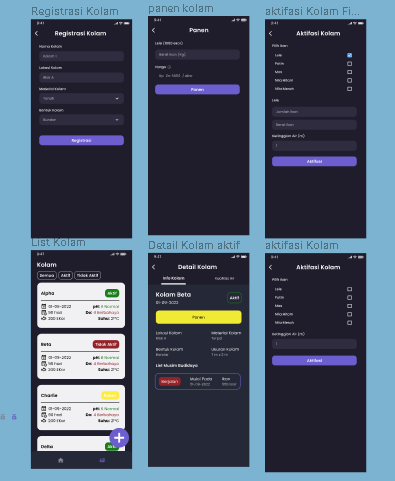
\includegraphics[keepaspectratio, width=4cm]{gambar/mockupsprint2}
	\caption{\textit{Mock-up UI List kolam, Registrasi kolam, Detail kolam, Aktivasi dan Deaktivasi kolam}}
	\label{gambar:mockupsprint2}
	\end{figure}

	\item{\textit{Class Diagram}}
	
	Class Diagram menggambarkan kelas-kelas yang akan dipakai oleh sistem. Umumnya terdapat 3 kelas pada setiap module yaitu class model, controller, dan view. Pada sprint-2 penelitian kali ini penulis membuat 4 class yaitu model yang berwarna biru, view berwarna oranye, controller yang berwarna hijau, dan service yang berwarna kuning.
	 
	 \begin{figure}[H]
	 \centering
	 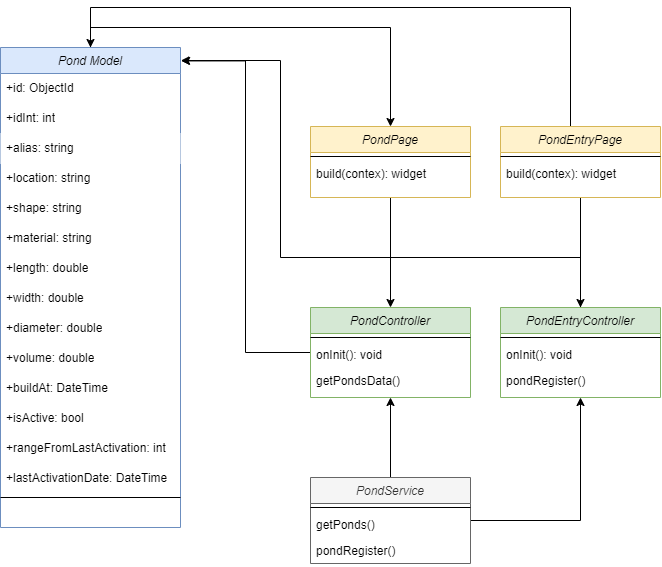
\includegraphics[keepaspectratio, width=6cm]{gambar/pondcd}
	 \caption{\textit{Class Diagram Fitur Koam Sprint-2}}
	 \label{gambar:pondcd}
	 \end{figure}

	 \begin{figure}[H]
	 \centering
	 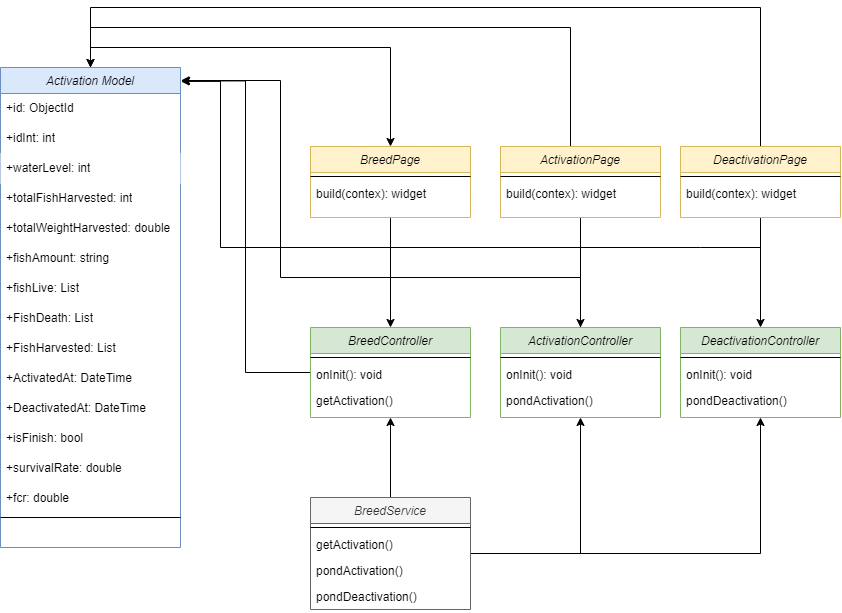
\includegraphics[keepaspectratio, width=6cm]{gambar/activationcd}
	 \caption{\textit{Class Diagram Fitur Aktivasi dan Deaktivasi Sprint-2}}
	 \label{gambar:activationcd}
	 \end{figure}

	\item{\textit{Menerapkan mockup-UI  halaman list kolam, registrasi kolam, detail kolam, aktivasi dan deaktivasi kedalam code flutter}}
	
	Setelah \textit{mock-up UI  halaman list kolam, registrasi kolam, detail kolam, aktivasi dan deaktivasi} dibuat, akan dilakukan pengimplementasian \textit{mock- up UI} ke dalam aplikasi menggukan flutter. Berikut adalah source code dari implementasi halaman list kolam, registrasi kolam, detail kolam, aktivasi dan deaktivasi yang terdapat pada lampiran 3 dan menghasilkan output halaman sebagai berikut

	\begin{figure}[H]
	\centering
	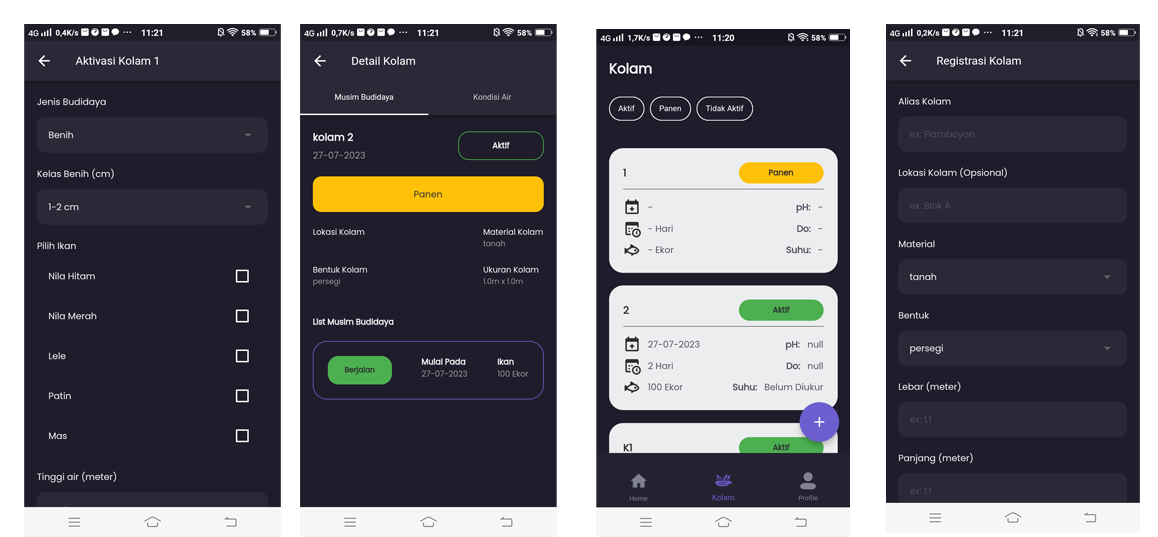
\includegraphics[keepaspectratio, width=8cm]{gambar/sssprint2}
	\caption{\textit{Output dari code pada sprint 2}}
	\label{gambar:sssprint4}
	\end{figure}

\item{Analisis \textit{User Experience}} 
 
pada halaman halaman list kolam terdapat card yang berisi informasi yang berguna bagi para pembudidaya untuk melakukan pemantauan terkait aktivitas yang terdapat pada masing-masing kolam. Sementara pada halaman registrasi kolam, pembudidaya harus memasukan data yang diperlukan untuk menambahkan kolam sesuai dengan kesepakatan saat meeting. Lalu pada halaman detail kolam terdapat data kolam terkait dan list musim budidaya yang telah berjalan di kolam tersebut. Sama halnya dengan aktivasi dan deaktivasi pembudidaya harus memasukan data yang diperlukan sesuai dengan kesepakatan saat meeting.


\item{Sprint 2 Review dan Sprint 3 Planning}

Sprint 2 diakhiri dengan melakukan weekly meeting pada hari selasa dengan agenda melakukan review dan testing terkait hasil sprint 2 dan melakukan planning untuk sprint 3 dengan rincian:
\begin{enumerate}
	\item{\textit{Review dan Testing hasil dari sprint 2}}

	Telah dilakukan review dan testing oleh penulis selaku developer dengan Scrum Master. Setelah dilakukan testing, Scrum Master menyimpulkan bahwa penerapan fitur pada halaman list kolam, detail kolam, aktivasi kolam, deaktivasi kolam telah berjalan dengan baik namun belum di integrasikan dengan data dari API sehingga akan dilanjutkan kedalam sprint berikutnya.

	\item{\textit{Sprint Planning untuk Sprint 3}}
	
	Planning untuk sprint 3 yakni membuat fitur pemberian pakan pada aplikasi \textit{Assistive Aquaculture Breeding Management}.
\end{enumerate}
\end{enumerate}